\chapter{Background}\label{chapter:background}

This section aims on providing a general overview of the various tools that were used in this work. In particular, the chosen FaaS platform as well as the employed edge devices needed to construct the experimental cluster will be introduced.

\section{Docker}
\textit{Docker} is an Open-Source containerization platform developed by Docker Inc. which enables software developers to bundle an application together with any associated configuration files and other dependencies, which have to be available at runtime in order to appropriately operate the packaged software, into Docker images. In the context of containerization, images contain an isolated filesystem and are standalone, executable software packages that act as an immutable blueprint for so-called containers, which are created once the respective image is executed. Containers are seperate, isolated processes that run on the host system and can be seen as the direct counterpart of Virtual Machines (VMs) due to the fact that they differ substantially in their characteristics and the way they function. For instance, containers are more lightweight and efficient because they utilize the kernel of the host's operating system (OS) instead of booting their own dedicated operating system, which results in a significant reduction of overhead and startup time. Furthermore, containers are highly portable because they only have to be created once in order to be deployed to any platform or environment as they are abstracted away from the OS of the host they run on. For example, Docker can be installed on Windows, Linux and macOS which makes it possible to deploy a containerized application to any of today's most common operating systems. Additionally, containerization completely eliminates the common problematic situation known from traditional software development where the software in question works in a certain environment, but falls into a faulty state when deployed to a different environment, due to the encapsulation of the application. Consequently, this accelerates productivity as it allows for a reproducible environment due to the fact that a container always behaves in the same way and is independent of the target platform and its surrounding. Lastly, Docker images can easily be shared with other developers by publishing it to an image registry such as Docker's \textit{DockerHub}, which is the world's largest repository service. 

The main component of Docker is the Docker Engine, which is a container runtime that acts as a client-server application and provides the following core features:

\begin{enumerate}
    \item \textit{Docker Daemon}: The Docker Daemon \textit{dockerd} is a persistent process that can be seen as the control plane of Docker. It is responsible for managing images, containers and other docker-related resources.
    \item \textit{Docker Engine API}: The Docker Engine offers a public RESTful API, which specifies interfaces that other programs can use in order to instruct the Docker daemon. These APIs can be accessed by any HTTP client.
    \item \textit{Command Line Interface (CLI)}: The Docker CLI named \textit{docker} acts as a client program that uses the provided APIs in order to communicate with the Docker daemon and can thus be used in order to build images, create or delete containers, pull an image from or push an image to a registry and more~\parencite{docker-engine}.
\end{enumerate}

Even though much of today's software is only required to run on x86-64 based computers, the situation of having to support different types of system architectures like ARM32v7 or its 64-bit based successor called ARM64v8 is not uncommon, especially when developing IoT applications that are targeted at a wide range of heterogeneous devices. To this end, Docker supports multi-architecture builds for Docker images, which enables application developers to generate and publish multiple versions of a specific image at once, while each one is dedicated to a specific processor architecture. After these images have been uploaded to an image registry, any device that has Docker installed is able to automatically pull the specific image that targets its architecture.


\section{Kubernetes}
\textit{Kubernetes} is a famous Open-Source container orchestration tool first introduced by Google, which is designed to automate the deployment, load balancing, scaling and management of containerized applications. Containers run inside a so-called \textit{Pod} which is the smallest deployable unit provided by Kubernetes. Since it is a cluster-based software, it is typically used in a multi-node production environment in which each node performs the task of either the Master or Worker. While the former acts as the cluster's decision maker by hosting the master components of a cluster such as the \textit{kube-scheduler}, which is responsible for assigning a target node to newly created pods, or the key-value based backup store \textit{etcd} which incorporates all data of a cluster, the latter maintains the pods which are components of the application workload by communicating with the master nodes by the help of a running agent called \textit{kubelet} in order to take corresponding instructions. Hence, the application containers managed by Kubernetes are eventually deployed to a cluster's worker nodes~\parencite{k8s-components}. As a result, the architecture of Kubernetes guarantees a great extensibility due to the fact that an existing cluster can easily be scaled by adding more worker nodes. Additionally, a cluster can be made highly-available and fault tolerant by extending it accordingly.\\
Kubernetes supports a wide range of container runtimes such as \textit{containerd} or any implementation of the Kubernetes Container Runtime (CRI) like CRI-O~\parencite{k8s-components}. Even though Docker has recently been removed from the list of supported runtimes, applications that have been containerized using Docker can still be deployed to Kubernetes as long as they don't directly depend on features or settings that are explicitly provided by Docker~\parencite{k8s-docker-drop}.

\section{Cluster Monitoring \& Data Visualization}
\subsection{Prometheus}
\textit{Prometheus} is an Open-Source, cutting-edge monitoring system that enables administrators to effectively supervise a system's infrastructure and associated applications. It is well known for its poll-based data collection model which regularly scrapes metrics over HTTP from the services being monitored, which are usually referred to as \textit{targets}, using a configurable time interval. Any data collected by a successful scrape is stored in a time-series database, which enables Prometheus to keep track of changes of the individual metrics over time. For the purpose of data selection and performing operations on the data, Prometheus provides an own query language called \textit{PromQL} which defines a wide range of functions that can be utilized in query expressions. Furthermore, it allows to define certain alert rules that are based on the collected data in order to trigger an alert once a specific condition defined in those rules is met. This allows for sending automatic notifications to administrating staff, which can then act appropriately based on what kind of alert has been triggered.\\
Generally, there is already a comprehensive amount of applications that natively expose metrics in the format expected by Prometheus. For any cases where this does not apply, a so-called data exporter can be employed, which is responsible for fetching data from third-party systems and transforming them into metrics that can be processed by Prometheus. To this end, client libraries that are available for a variety of programming languages can be made use of in order to implement such an exporter for a specific application.

\subsection{Grafana}
\textit{Grafana} is a modern Open-Source data analytics \& visualization platform that offers the possibility to plot data, which can be obtained from a variety of different sources, in interactive, dynamic dashboards. Prometheus is one of the most commonly used data sources for Grafana, which qualifies it as another powerful component of a modern system monitoring toolchain. Due to the fact that it provides the opportunity to construct an arbitrary amount of dashboards that are highly configurable, users are able to achieve a visualization of their data that satisfies individual requirements.

\section{OpenFaaS}
OpenFaaS is one of the most popular Open-Source FaaS platforms and is suitable for production-ready, large-scale applications due to the fact that it can be deployed to the commonly known industrial-strength container orchestration systems Kubernetes and OpenShift. On the other hand, it offers an alternative designed for less complex and comprehensive projects named \textit{faasd}, which is a lightweight version of OpenFaaS that offers the opportunity to avoid the complexity of Kubernetes~\parencite{openfaas-deployment}. OpenFaaS is very straightforward and easy to use as serverless functions can be written in any programming language - the only requirement is packaging the application as a container image that complies with the format defined by the \textit{Open Container Initiative} (OCI) and publishing it to an image registry~\parencite{openfaas-intro}. Afterwards, the function can be deployed and invoked by the \textit{API Gateway} which can be accessed via its REST API, the provided Command Line Interface named \textit{faas-cli} or the Web UI. Additionally, invocations can also be triggered by a scheduled cron-job or by third-party systems such as message brokers like \textit{Apache Kafka} or \textit{RabbitMQ}. For the latter, OpenFaaS offers so-called connectors that map a certain topic to multiple functions, which allows for triggering an arbitrary amount of functions once a new message of the specific topic was received by the broker~\parencite{openfaas-triggers}. Figure 2.6 provides an overview of the overall function invocation procedure and the individual components that are involved.

\begin{figure}[h]
    \centering
    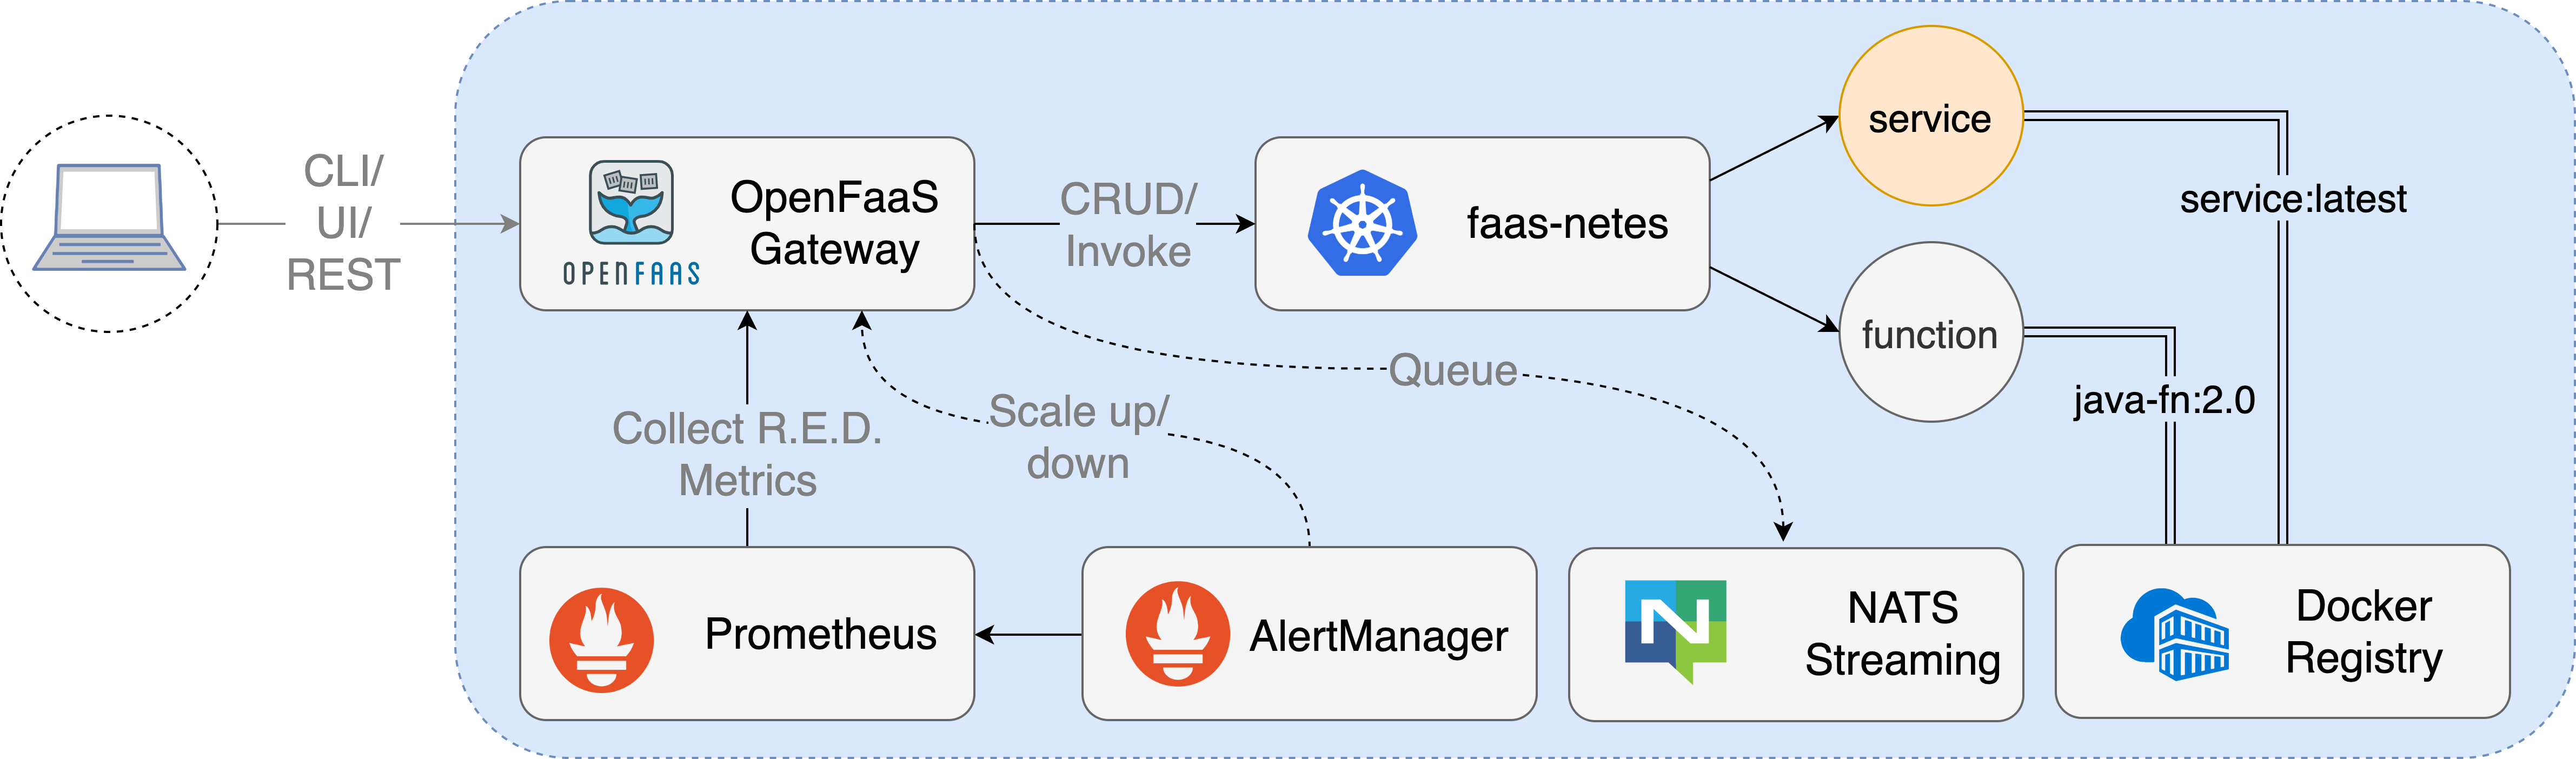
\includegraphics[width=1\textwidth]{./figures/of-workflow.png}
    \caption{Interaction with the OpenFaaS API Gateway~\parencite{openfaas-stack}}
    \label{fig:openfaas-gateway}
\end{figure}

\section{Function Delivery Network}
Current FaaS platforms are restricted to homogeneous clusters and serverless functions, which is a significant limitation due to the fact that heterogeneity of compute clusters and computational resources is steadily increasing in today's cloud applications. For instance, an IoT application may utilize an IoT cloud that consists of a cluster of multiple microcontroller-based systems, which might use different processor architectures and substantially differ in their hardware equipment, and another cluster composed of powerful Virtual Machines (VMs), which is responsible for handling the computationally more intensive tasks. Consequently, serverless functions that demand a significant amount of compute and data resources should be scheduled in an appropriate cluster that is able to fulfill these requirements. Additionally, it is important to mention that, due to hardware constraints present on edge devices, it can not be guaranteed that a certain FaaS platform can actually run on them, which prevents the use of a homogeneous FaaS platform over multiple heterogeneous clusters ~\parencite{fdn}.
In summary, this implies the need for the possibility to deploy heterogeneous FaaS platforms in heterogeneous clusters and to schedule the execution of serverless functions based on their individual resource requirements. To this end, data access behavior such as access latency should be taken into account in an effective manner in order to optimally utilize the available resources.
\\
The Function Delivery Network (FDN) is a distributed network of target platforms, which is designed to extend the concept of serverless computing based on FaaS in order to overcome the mentioned limitations. It is highly versatile as it can be connected with a wide range of different target platforms due to the fact that it integrates with clusters that are dedicated for a multitude of purposes such as cloud and edge computing as well as High Performance Computing (HPC). Additionally, the FDN supports multiple FaaS providers like Apache OpenWhisk, OpenFaaS, AWS Lambda or Google Cloud Functions.\\
It supplies FDaaS by requiring the user to provide an application configuration file, which describes the individual functions, APIs, permissions and other associated configuration. This file is subsequently passed to the following core components of the FDN:

\begin{enumerate}
    \item \textit{Deployment Generator}: This unit annotates the file with a deployment configuration for the specific application based on knowledge that was either previously collected by the FDN or externally provided by an expert.
    \item \textit{Control Plane}: This is the main component of the FDN. It is responsible for managing the access control which includes authentication and authorization as well as for monitoring the overall infrastructure and applications. Additionally, it handles data placement and the scheduling of function invocations based on the annotated deployment specification.
\end{enumerate}

The decisions that are made by the Control Plane at runtime regarding function scheduling and data placement depend on several behavioral models, which are created during the execution of an application by another component called \textit{Behavioral Modeling}. These models are continuously updated in an online learning fashion by extracting knowledge from data that is regularly collected by the FDN from the application's functions~\parencite{fdn}.

\section{Edge-Enabled IoT Devices}

\subsection{Raspberry Pi 3 Model B v1.2}

\begin{figure}[h]
    \centering
    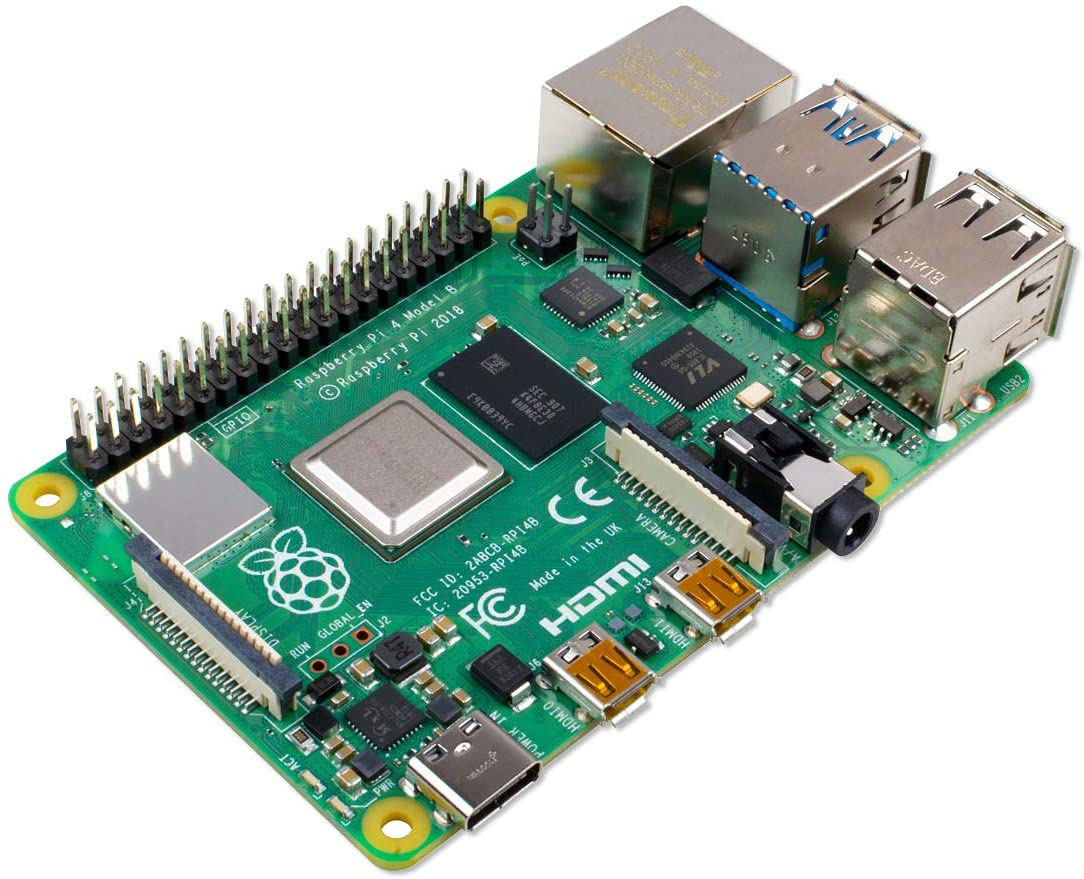
\includegraphics[width=0.30\textwidth]{./figures/mesh}
    \caption{The Raspberry Pi 3 Model B v1.2}
    \label{fig:raspberry-pi}
\end{figure}


The Raspberry Pi 3 Model B v1.2 is the earliest model of the third generation of the Raspberry Pi, which is probably the most commonly known single-board computer in the world due to its affordability. It was developed by the british Raspberry Pi Foundation and is equipped with 1 GB of LPDDR2 RAM and a Cortex-A53 Quad-Core ARM64v8 processor with a Broadcom BCM2837 chipset that operates at 1.2 GHz. Even though the installed chip implements the 64-bit instruction set, the use of a 64-bit based operating system hardly offers a performance boost due to the low amount of available RAM which is why the Raspberry Pi used in this work runs a 32-bit Raspbian OS. In order to operate the Raspberry Pi a power supply of 5V at 2.5A via Micro USB is required~\parencite{raspberry-pi-intro}.

\subsection{NVIDIA Jetson Nano Developer Kit}

\begin{figure}[h]
    \centering
    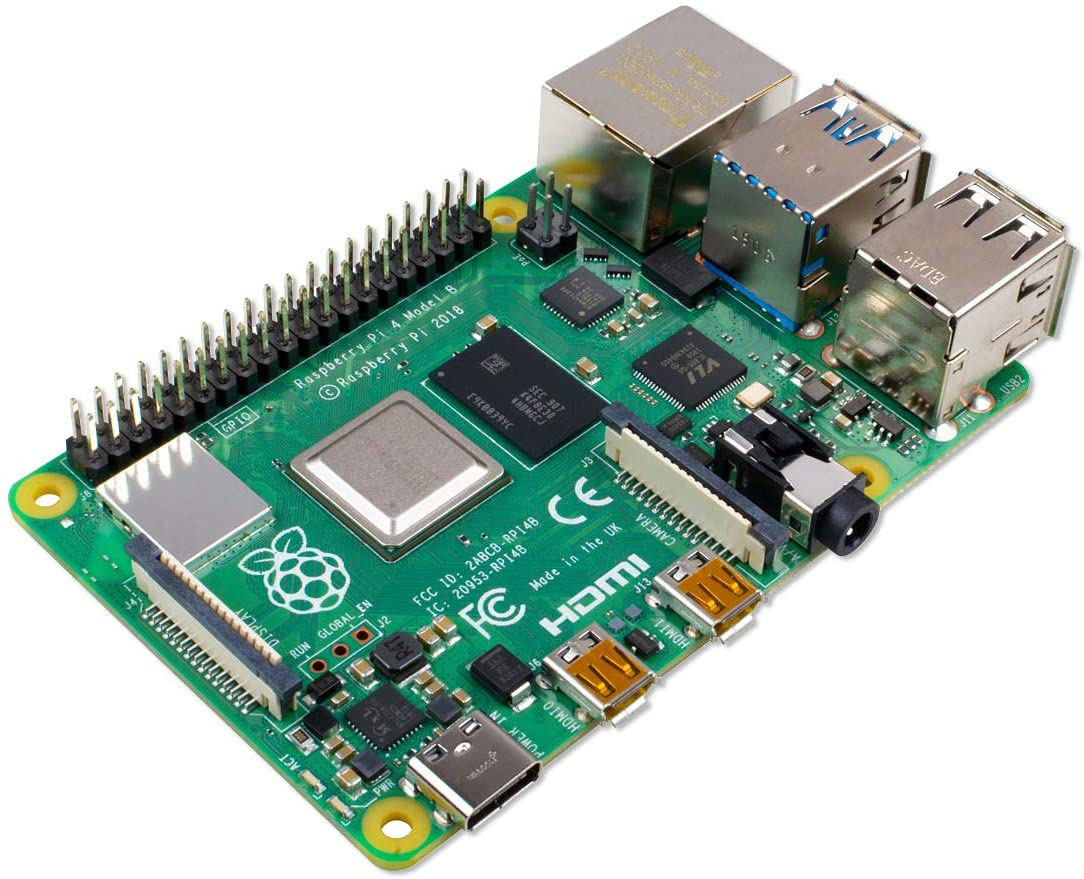
\includegraphics[width=0.30\textwidth]{./figures/mesh}
    \caption{The NVIDIA Jetson Nano Developer Kit}
    \label{fig:jetson-nano}
\end{figure}

The NVIDIA Jetson Nano Developer Kit is a performant single-board computer developed by the NVIDIA Corporation and is primarily designed for the purpose of developing and executing AI applications. To this end, it is provided with a Cortex-A57 Quad-Core ARM64v8 CPU that runs at 1.43 GHz as well as with an NVIDIA 128-core NVIDIA Maxwell GPU. Additionally, the Jetson Nano Developer Kit has access to 4 GB of LPDDR4 RAM and requires a slightly higher power supply of 5V at 2.5A - however, supplying up to 4A is recommended.~\parencite{jetson-nano-devkit-manual}

\subsection{Google Coral Dev Board}

\begin{figure}[h]
    \centering
    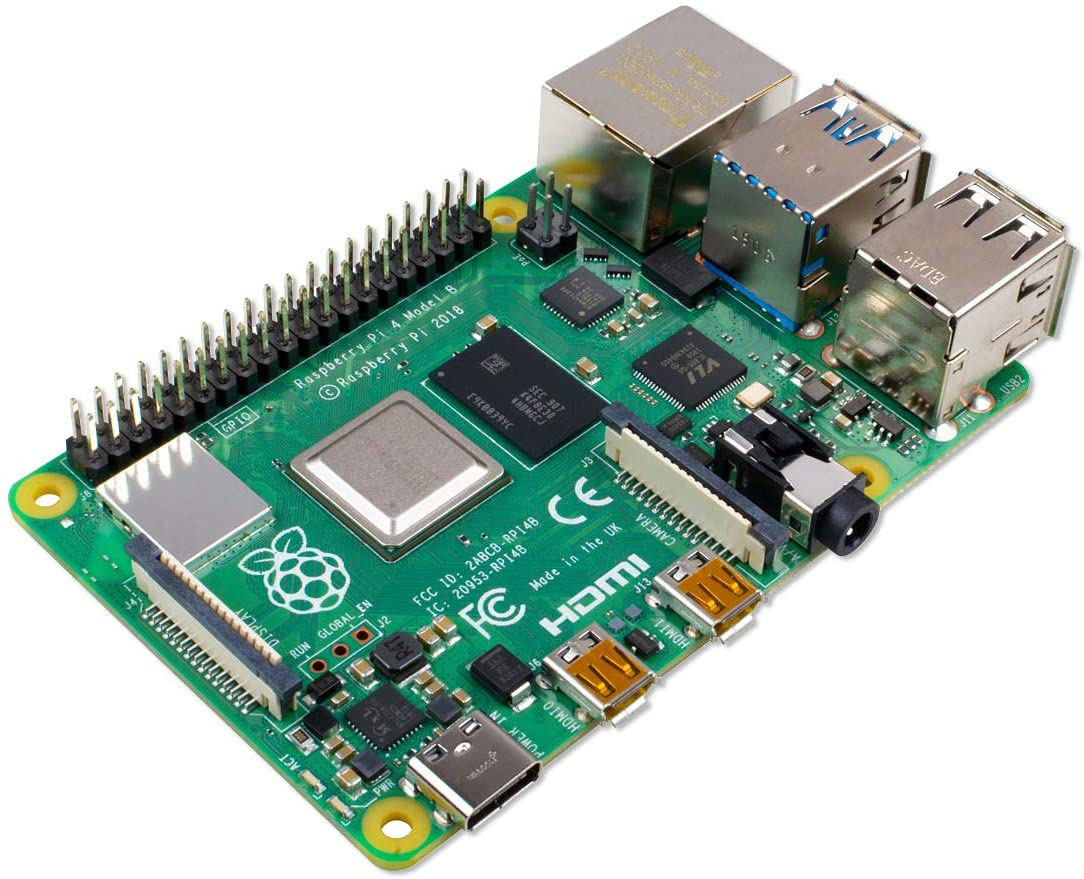
\includegraphics[width=0.30\textwidth]{./figures/mesh}
    \caption{The Google Coral Dev Board}
    \label{fig:coral-dev-board}
\end{figure}

The Coral Dev Board is a single-board computer designed to facilitate machine learning inference and embedded system development. Next to a Vivante GC7000Lite GPU and a Cortex-A53 Quad-Core ARM64v8 processor that operates at up to 1.5 GHz, it is equipped with an Edge TPU coprocessor developed by Google which significantly leverages the performance. Moreover, it is provided with 1 GB of LPDDR4 RAM and demands a power supply of 5V at around 2-3A.~\parencite{coral-dev-board-manual}

\subsection{ODROID-XU4}

\begin{figure}[h]
    \centering
    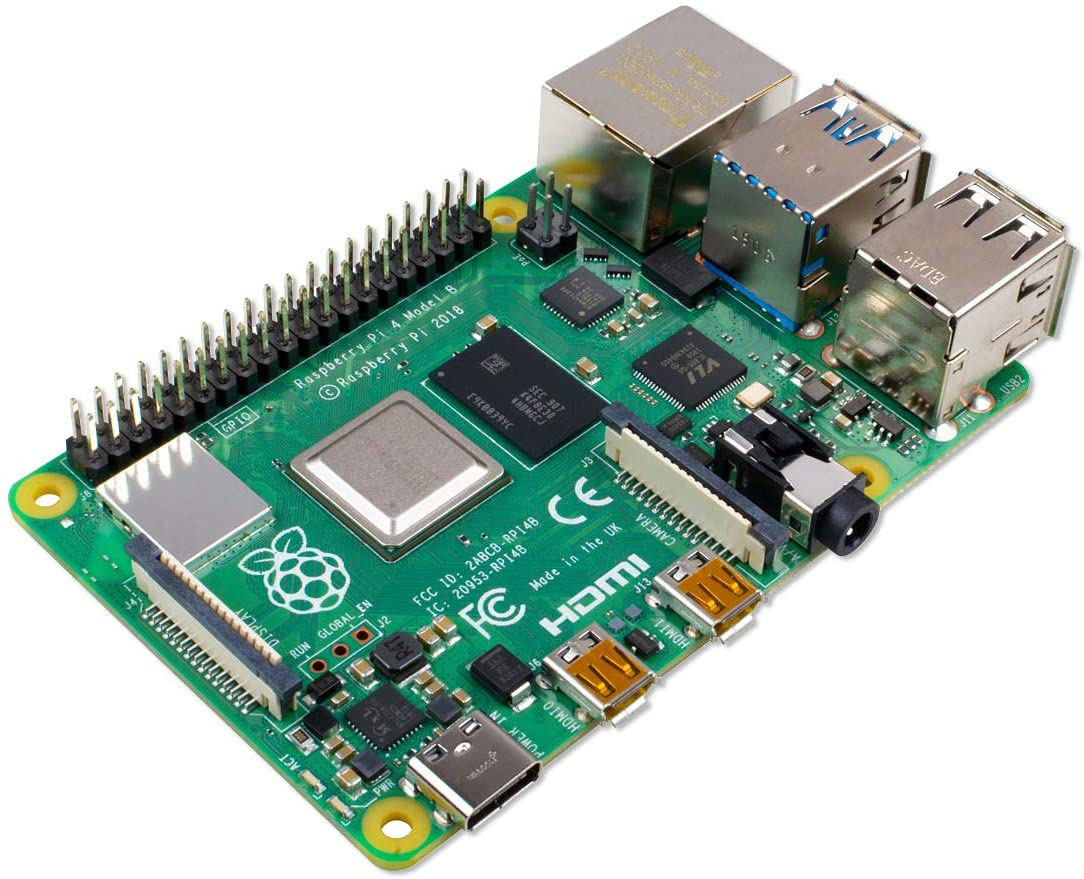
\includegraphics[width=0.30\textwidth]{./figures/mesh}
    \caption{The Odroid XU4}
    \label{fig:odroid-xu4}
\end{figure}

The ODROID-XU4 is a powerful single-board computer manufactured by Hardkernel, which is specifically well suited for developing software designed for the Android operating system. It comes with a SAMSUNG Exynos 5422 Octa-Core ARM32v7 CPU running at 2 GHz, an integrated Mali-T628MP6 GPU and 2 GB of LPDDR3 RAM. Even though the board consumes less than 1A in the most cases, providing a power source supplying 5V at 4A is recommended in order to operate the XU4.~\parencite{odroid-xu4-manual}

\subsection{XILINX PYNQ-Z1}

\begin{figure}[h]
    \centering
    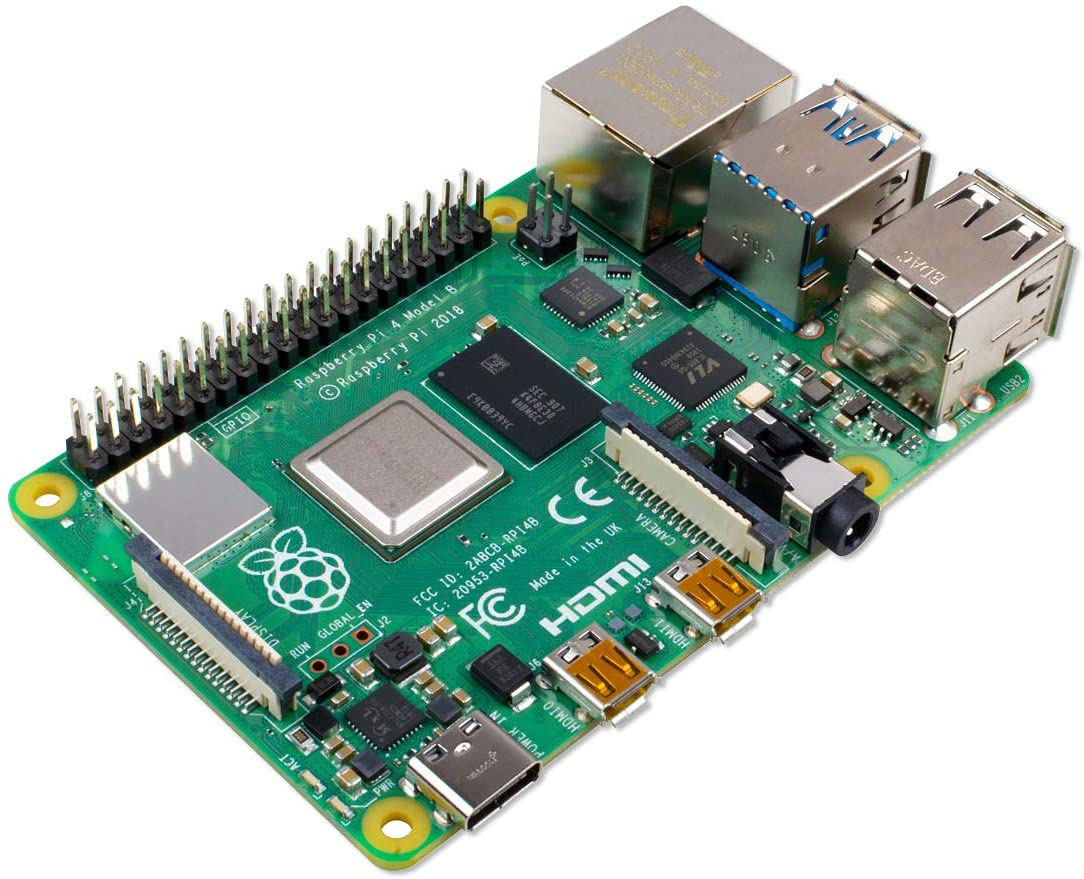
\includegraphics[width=0.30\textwidth]{./figures/mesh}
    \caption{The XILINX PYNQ-Z1}
    \label{fig:xilinx-pynq-z1}
\end{figure}

The XILINX PYNQ-Z1 is a general purpose single-board computer manufactured by Digilent. It is designed to be used with the Open-Source framework PYNQ, which is based on the programming language Python and facilitates prototyping and embedded software development for the individual XILINX platforms. The board is supplied with 512MB of DDR3 RAM and a Cortex-A9 Dual-Core ARM32v7 processor which operates at up to 650 MHz. At the bare minimum, the PYNQ-Z1 can be powered via USB 2.0, which, according to the specifications, provides 5V at up to 0.5A. For more complex applications, an external source supplying 7V at the minimum and 15V at the maximum should be used~\parencite{pynq-z1-manual}.